\documentclass{article}
\usepackage[T1]{fontenc}
\usepackage{lmodern}
\usepackage{graphicx}
\usepackage{amsmath,amssymb}
\usepackage[a4paper,margin=2cm]{geometry}
\usepackage[absolute,overlay]{textpos}
\setlength{\TPHorizModule}{1mm}
\setlength{\TPVertModule}{1mm}
\usepackage[indonesian]{babel}
\usepackage{hyperref}
\setlength{\emergencystretch}{2em}
% unit: Halaman 9

\begin{document}

% === Halaman 9 (llm) ===

\vspace{180.28mm}

\begin{itemize}
  \item Perbandingan: top 10 huruf yang paling sering muncul dalam Bahasa Indonesia:
\end{itemize}
\vspace{5mm}

% deskripsi: Tabel frekuensi kemunculan 10 huruf teratas dalam Bahasa Indonesia beserta persentase peluangnya.
% bbox normalisasi: [0.3670, 0.2160, 0.5210, 0.8230]
\begin{textblock*}{32.34mm}(77.07mm,64.15mm)
\noindent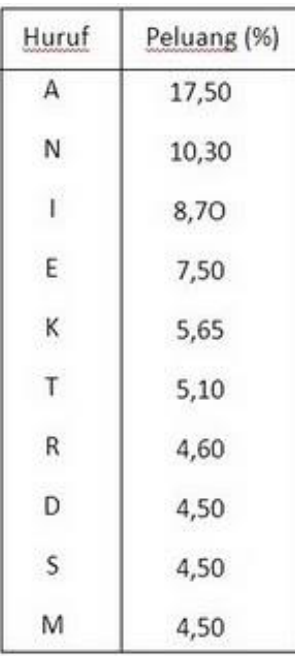
\includegraphics[width=32.34mm,height=180.28mm]{../../images/llm/page_009_img_01.png}%
\end{textblock*}

\end{document}
